
\section{Darbų pasiskirstymas mėnesiais intervalais}

\begin{figure}[htb]
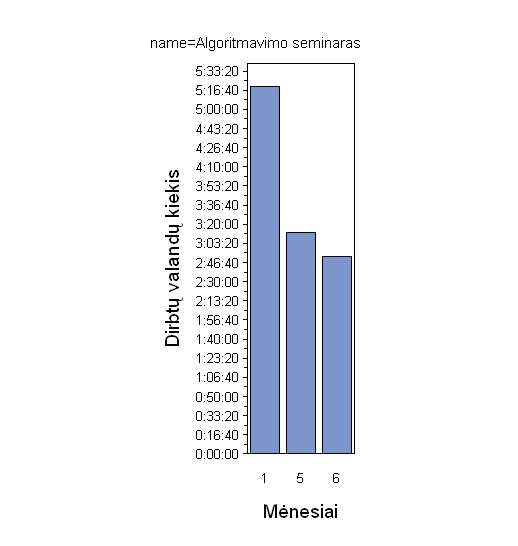
\includegraphics[width=0.9\linewidth]{images/months/Algoritmavimo_seminaras.png}
\caption{Algoritmavimo seminaras}
\label{fig:algoritm}
\end{figure} 

\begin{figure}[htb]
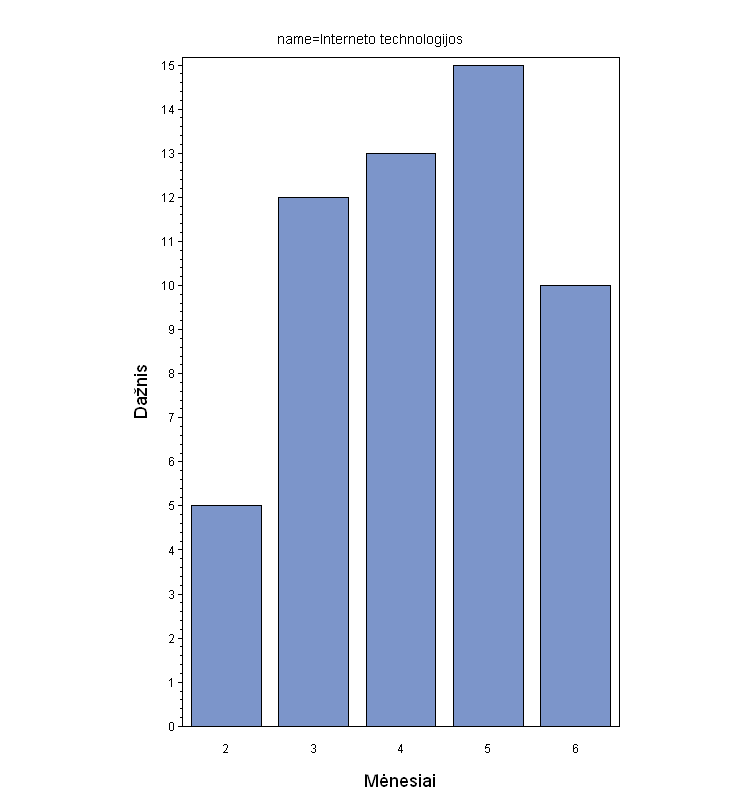
\includegraphics[width=0.9\linewidth]{images/months/Interneto_technologijos.png}
\caption{Interneto technologijos}
\label{fig:it}
\end{figure}


\begin{figure}[htb]
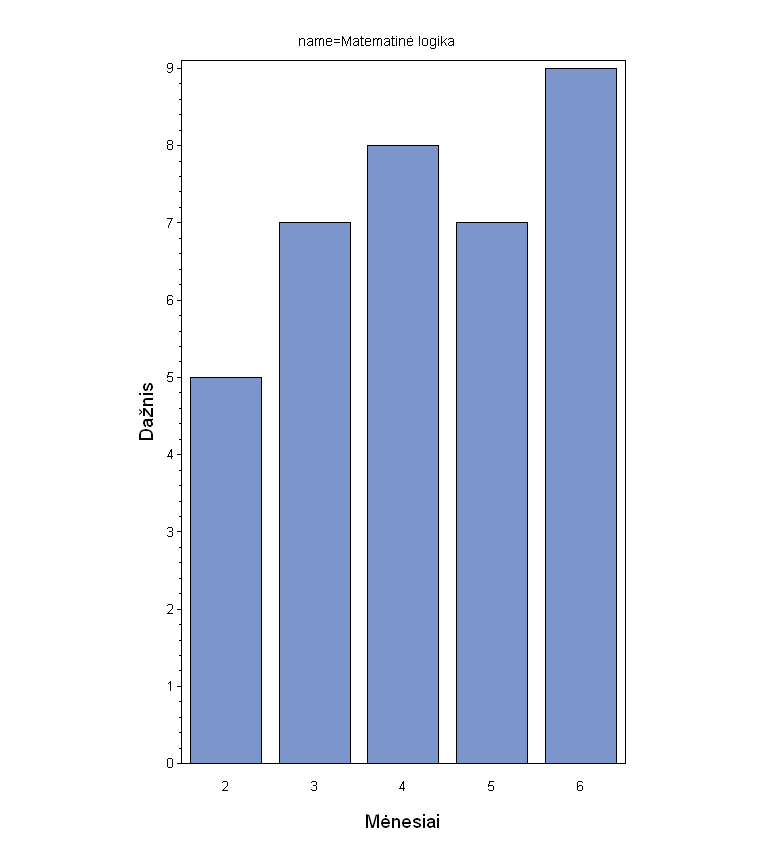
\includegraphics[width=0.9\linewidth]{images/months/Matematine_logika.png}
\caption{Matematinė logika}
\label{fig:matlog}
\end{figure}

\begin{figure}[htb]
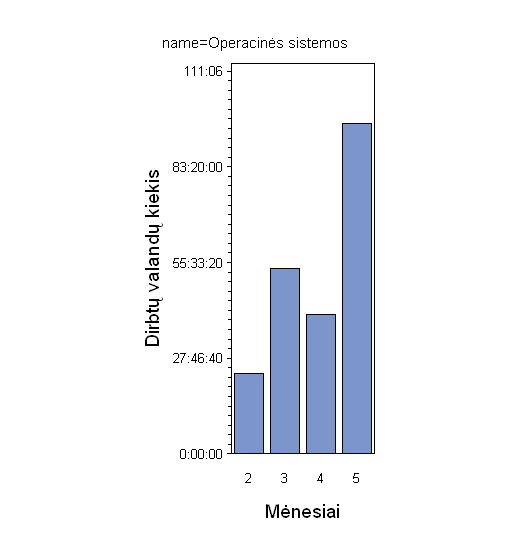
\includegraphics[width=0.9\linewidth]{images/months/Operacines_sistemos.png}
\caption{Operacinės sistemos}
\label{fig:os}
\end{figure}

\begin{figure}[htb]
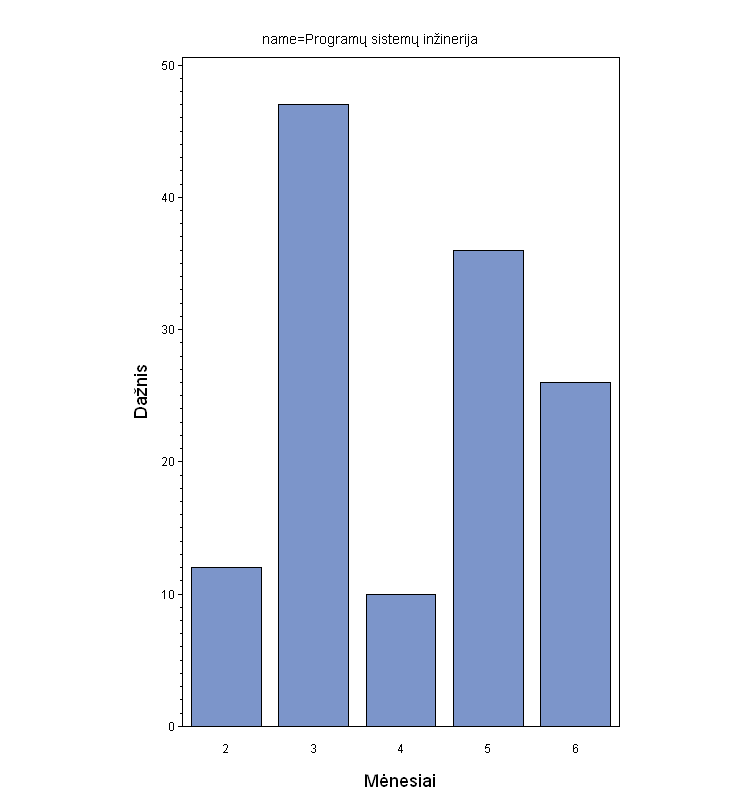
\includegraphics[width=0.9\linewidth]{images/months/Programu_sistemu_inzinerija.png}
\caption{Programų sistemų inžinerija}
\label{fig:psi}
\end{figure}

\begin{figure}[htb]
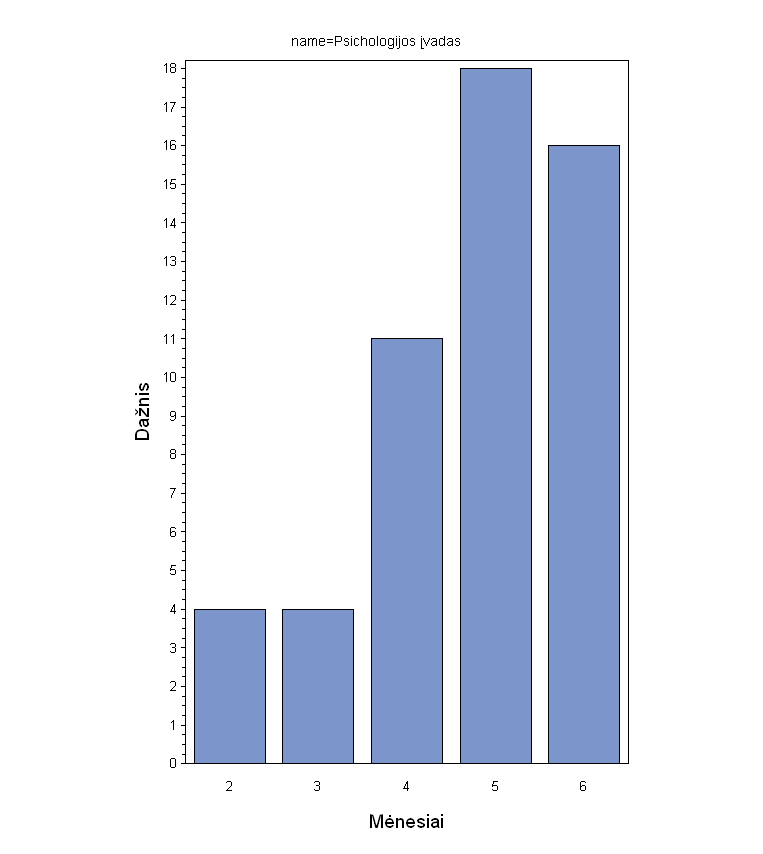
\includegraphics[width=0.9\linewidth]{images/months/Psichologijos_ivadas.png}
\caption{Psichologijos įvadas}
\label{fig:psicho}
\end{figure}

\begin{figure}[htb]
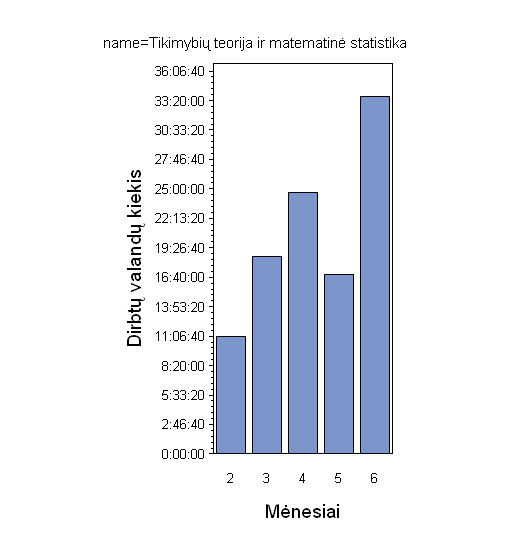
\includegraphics[width=0.9\linewidth]{images/months/Tikimybiu_teorija_ir_matematine_statistika.png}
\caption{Tikimybių teorija ir matematinė statistika}
\label{fig:statistika}
\end{figure}


\begin{figure}[htb]
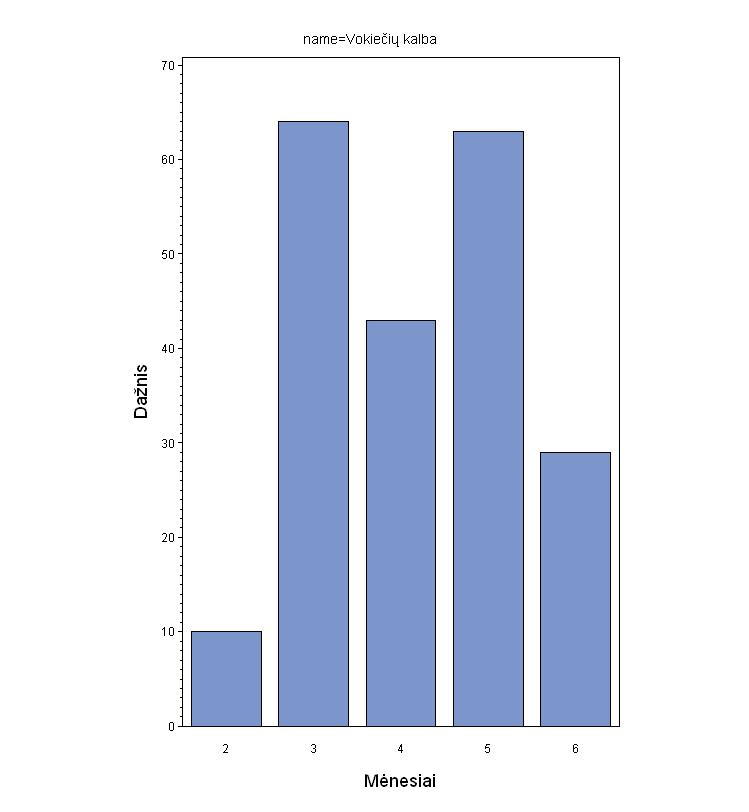
\includegraphics[width=0.9\linewidth]{images/months/Vokieciu_kalba.png}
\caption{Vokiečių kalba}
\label{fig:vokieciu}
\end{figure} 